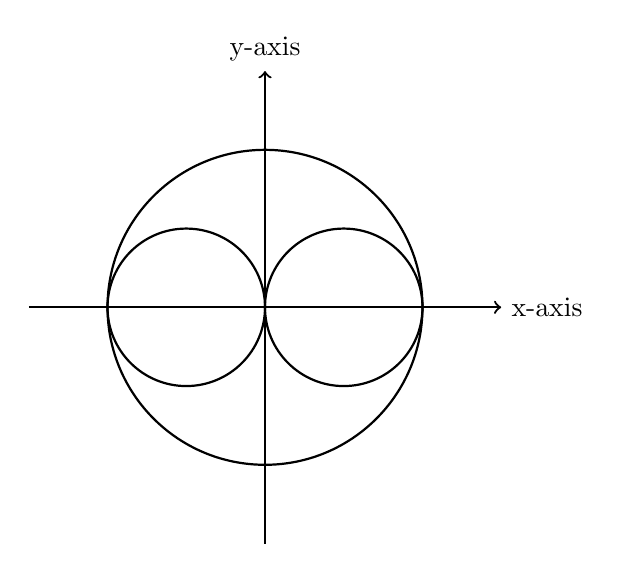
\begin{tikzpicture}

    % Define the radius of the large circle
    \def\R{2} % Radius of the large circle

    % Draw the large circle centered at the origin
    \draw[thick] (0,0) circle (\R);

    % Draw the two smaller circles
    % Each smaller circle has a radius of \R/2 and is positioned to the left and right
    \draw[thick] (-\R/2,0) circle (\R/2); % Left smaller circle
    \draw[thick] (\R/2,0) circle (\R/2);  % Right smaller circle

    % Draw the x-axis and y-axis
    \draw[->, thick] (-\R-1,0) -- (\R+1,0) node[anchor=west] {x-axis};
    \draw[->, thick] (0,-\R-1) -- (0,\R+1) node[anchor=south] {y-axis};

\end{tikzpicture}

